\documentclass[14pt]{article}
\usepackage{graphicx}
\usepackage{xcolor}
\usepackage{ragged2e}
\usepackage{polski}
\usepackage{tabularx}
\newcolumntype{Y}{>{\centering\arraybackslash}X}

\title{\textbf{Piekielny rodowód}}
\author{Akt I}
\date{Narodziny demona}

\begin{document}

\pagenumbering{gobble} 
\begin{figure}
    \centering
    
\includegraphics[width=1\textwidth]{devil.png}
\end{figure}
\maketitle
\newpage
\pagenumbering{arabic}

\centering
\section*{(1) PROLOG}
\RaggedRight
Ciepły wieczór. Jesteście w portowym mieście Alegard. Siedzicie w ogrodzie za karczmą. Popijacie piwo z kufla, śmiejecie się, bawicie. Ravn słyszy z oddali skrzekot ptaka. Wyciąga rękę a po chiwli na jego ramieniu ląduje kruk. Wyciąga z jego łapki kartkę, po czym kruk odlatuje. Ravn czyta z zaciekawieniem wiadomość. Po czym wstaje i głośnym tonem wypowiada "Zajebiście". Gdy reszta graczy zainteresuje się zachowaniem diabiła Ravn mówi co wyczytał w wiadomości:
\begin{itemize}
    \item[\textbf{R:}] Dostałem sympatyczną wiadmość. Mamy zlecenie na odzyskanie piekielnego artefaktu. Dają w chuj kasy.
\end{itemize}
Oczywiście brak zgody nie wchodzi w grę. Ravn przedstawia co się dowiedział z listu:
\begin{itemize}
    \item[\textbf{R:}] Za dużo się nie dowiedziałem. Ogólnie w mieście jest znawca i kolekcjoner takich rzeczy. Agon Dusiciel, były najemnik, potem pijak, aktualnie szlachcić. Ktoś ukradł mu artefakt i chce żebyśmy go odzyskali. Postaram do rana zdobyć informacje.
\end{itemize}
Ravn wstaje i wchodzi. Reszta ma czas dla siebie.
\newpage

\Centering
\section*{(2) PRZYGOTOWANIA}
\RaggedRight
Gracze budzą się. Ravn czeka w głównej izbie na resztę. Gdy pojawią się przedstawia całkowity plan działania:
\begin{itemize}
    \item[R:] Musimy zdobyć informacje na temat tego artefaktu. Możemy poszukać w kilku miejscach. Slamsy, rynek, port. Warto też zajrzeć do naszego pracodawcy, może nam coś podpowie. Ja uruchomię swoje kontakty i postaram się zdobyć więcej informacji.
\end{itemize}
Gracze dogadują się gdzie chcą iść. Następnie Ravn rozdaje mapy dla graczy. Na każdej z nich zaznaczył dom Agona Dusiciela. Gracze idą szukać informacji.

\Centering
\section*{(3) DOM AGONA}
\RaggedRight
Gracze podchodzą do domu szlachcica. Na wejściu wita ich strażnik, nie koniecznie w miły sposób. Gracze dostają się do domu, nie ważne jak. Wchodzą do głównego holu gdzie stoi Agon (PATRZ OPIS POSTACI). Wita graczy i pyta czego szukacie u niego w domu. Na pytanie o artefakt odpowiada:
\begin{itemize}
    \item[-] Jest to pradawny artefakt z głową demona. Mówią że skrywa w sobie wiele tajemnic. Wczoraj w nocy ktoś się włamał do mojego domu i ukradł artefakt. Chcecie zobaczyć miejsce zdarzenia?
\end{itemize}
Jeżeli gracze zdecydują się odwiedzić miejsce włamania Agon zaprowadza ich do niego. \\
\vspace{5mm}
Agon wprowadza graczy do sali trofeu. Na miejscu podejrzanie kręci się lokaj Agona. Agon wygania go. Na ścianach wiszą różne artefakty, w gablotach widać czaszki demonów, szkielety piekielnych stworzeń. Na środku sali widać gablotę z rozbitą szybą i pustymi uchwytami na artefakt. \\
\vspace{5mm}
W trakcie rozmowy Agon będzie usilnie nakierowywać graczy na klasztor Łowców Piekieł.
\newpage

\Centering
\section*{(4) PORT}
\RaggedRight
Gracze wkraczają do portu. Nie widać nic ciekawego prócz karczmy, strażników oraz grupy kurtyzan.
\begin{itemize}
    \item[-] \textbf{KURTYZANY}
    Kurtyzany jedynie co powiedzą że ich nie obchodzą kradzieże tylko ile ktoś jest w stanie zapłacić za ich usługi. Jeżeli ktoś będzie chciał skorzystać z usług niech się tak stanie. Po stosunku prostytutka powie że za dodatową opłatą powie co wie.
    \item[-] \textbf{KARCZMA}
    W karczmie widać grupkę marynarzy którzy bawią się ile się da. Jeżeli gracze Stwierdzą do nich podejść i wypytywać zacznie się awantura i walka. Po walce bądź w trakcie do karczmy wkroczą strażnicy. Strażnicy karzą zapłacić grzywnę i wynosić się z karczmy.
    \item[-] \textbf{STRAŻNICY}
    Nie ważne jak bardzo gracze będą próbowali wydostać informacje ze strażników jedynie co usłyszą to żeby spierdalali.
\end{itemize}

\Centering
\section*{(5) RYNEK}
\RaggedRight
Na rynku słychać przekrzykujących się handlarzy, na mówinicy miejski krzykacz przekazuje najświeższe informacje. Na uboczu widać jak zakapturzony mężczyzna robi jakieś nie do końca legalne interesy.
\begin{itemize}
    \item[-] Jeżeli gracze podejdą do kikona ten za odrobinę złota zdradzi im informacje o statku "Wielka Anala". Jest to statek Łowców Piekieł, elitarnej grupy która zwalcza demony.
    \item[-] Jeżeli gracze podejdą do zakapturzonego mężczyzny ten szybko zacznie biec do ciemnego zaułku. Jeżeli złapią mężczyzne ten im zdradzi informacje o spotkaniu Łowców Piekieł i miejskiej straży przy młynie.
\end{itemize}
Jeżeli gracze zdobyli informacje o spotkaniu. Mogą się na nie udać pod młyn. Mogą starać podsłuchać rozmowę. Z rozmowy wynika że to nie oni ukradli artefakt, ale szukają go, ponieważ może wyczynić wiele złego. Możliwe że ukradł go Moira, szef tutejszego gangu.
\newpage

\Centering
\section*{(6) SLAMSY}
\RaggedRight
Gracze na wejściu do slamsów od razu zostają zaczepieni przez gangusów. Chcą zaprowadzić graczy do ich szefa. Gracze mogą pójść lub odmówić, wtedy gangusy będą chcieli wziąć ich siłą. \\ Jeżeli gracze zgodzą się na spotkanie, lub zostaną zaprowadzeni siłą spotkają się z Moirą, szefem gangu. \\ Jeżeli nie spotkają się z Moirą będą jedynie krążyć po slamsach bez celu. \\
\vspace{5mm}
Spotkanie z Moirą. Szef gangu przedstawia sytuacje. Mówi że to Łowcy ukradli artefakt i trzymają go na statku. Proponuje dwa razy tyle co zaproponował Agon. Mówi także że artefakt zamknięty jest w małym kufrze pod pokładem w magazynie. Gdy Moira kończy rozmowę widać jak dwóch chamów niesie dużą skrzynie. Jeden z nich ją upuszcza. Moira wstaje i krzyczy na swoich pracowników:
\begin{itemize}
    \item[M:] Kurwa mać. Mogli byście uważać. Wiecie jest tam coś BARDZO WAŻNEGO. 
\end{itemize}
Chamy podnoszą skrzynie, a gracze opuszczają lokal.

\Centering
\section*{(7) SPOTKANIE Z ZAKONEM}
\RaggedRight
Gracze którzy wychodzą ze slamsów napotykają Łowców Piekieł. Ci grzecznie się przedstawiają. Jeden z nich to Franz, głównodowodzący całej sytuacji. Uważają że to Moira ukradł artefakt. Wiedzą że gracze mają na niego zlecenie ale proszą aby zwrócili go dla zakonu. Proponują jedynie w zamian dozgonną wdzięczność.

\Centering
\section*{(8) CO DALEJ?}
\RaggedRight
Gracze mogą wrócić do Ravna, bądź na własną rękę pójść szukać artefaktu.
\newpage

\Centering
\section*{(9) STATEK}
\RaggedRight
Jeżeli gracze stwierdzą że chcą znaleźć artefakt na statku, będą musieli udać się do portu i poszukać statku "Wielka Anala". Nie trudno będzie znaleźć statek ponieważ jest to największy statek w porcie. Przed statkiem będzie stał ochroniarz. Gracze mogą użyć siły bądź sprytu. Sposób siłowy doprowadzi do walki na dolnym pokładzie. Sposób sprytny doprowadzi do akcji skradania na dolnym pokładzie. Akcja skradania może się nie udać i doprowadzić do walki. Gracze mogą znaleźć notatkę na stole kapitana która brzmi:
\begin{itemize}
    \item[] Nie wiem jak Agon dostał ten artefakt. Nie chcę wiedzieć nawet gdzie on to znalazł. Wiem na pewno że nie zrobi z tym nic dobrego. Mam nadzieję że jego lokaj coś z tym zrobi. W mieście artefaktem interesuje się Moira, lokalny żezimieszek. Tą sprawą ja się zajmę. Grupka patałachów dostała zlecenie na ten artefakt. Postaram się jakoś ich nasłać na Moire. Strażników też jakoś przekonam. Mam nadzieję że uda nam się odzyskać ten artefakt. Podpisane -Franz
\end{itemize}
Gracze mogą także trafić do magazynu. W magazynie znajdą jedynie beczki z jedzeniem i skrzynie z ubraniami. Następnie gracze decydują się gdzie się udać.

\Centering
\section*{(10) SIEDZIBA GANGU}
\RaggedRight
Przed siedzibą gangu siedzi ork ochroniarz. Gracze mogą go podejsć sprytem lub siłowo. Jeżeli gracze użyją siły w siedzibie gangu dojdzie do walki. Jeżeli użyją sprytu będą mogli przekraść się przez siedzibę. Mogą zostać odkryci co doprowadzi do walki. Jeżeli wejdą do biura znajdą notatke:
\begin{itemize}
    \item[] Nie wiem co te szmaciarze z zakonu kombinują ale na pewno nie zdobędą mojego artefaktu. Kosztuje wystaczająco dużo żebym mógł wynieść się z tego pierdolnika.
\end{itemize}
W magazynie znajdą jedynie beczki z piwem i kufer pełen drewnianych kutasów.
\newpage
\Centering
\section*{(11) PO RABUNKU}
\RaggedRight
Jeżeli gracze napadli na statek, przed wejściem będzie czekać na nich Moira. Jeżeli gracze napadli na siedzibę gangu, przed wejściem będzie czekać na nich Franz. Jeżeli gracze powiedzą co zdołali znlaeźć będą mieć sojusznika w finałowej walce. W innym wypadku będą musieli poradzić sobie sami. \\
Jeżeli udadzą się do domu Agona spotkają tam jedynie ledwo żywego lokaja. Powie im że Agon zabrał mu artefakt i udal się na polanę na zachód od miasta. Mówi też że trzeba się śpieszyć bo niedługo użyje artefaktu\\
Jeżeli gracze udadzą się do Ravna ten jedynie co powie że sytuacja jest chujowa. Po chwili słychać wielki wybuch, a do karczmy wbiega Franz. Mówi że Agon użył artefaktu i trzeba szybko go powstrzymać.

\Centering
\section*{(12) WALKA Z AGONEM}
\RaggedRight
Gracze docierają na polane. Jeżeli rytuał nie został jeszcze rozpoczęty gracze mogą spróbować przeszkodzić, bez skutku. Agan chwyci artefakt i użyje jego mocy. Nastąpi uwolnienie mocy, a Agon zamieni się w demona. Wykrzyczy że nie dacie rady go powstrzymać i zacznie się walka. Jeżeli rytuał został już rozpoczęty gracze zobaczą demona który wykrzyczy "Nie dacie pokonać mnie Agona" i rozpocznie się walka. Nie ważne jak walka się potoczy, Agon znika Wykrzykując coś w jezyku piekielnym. Po walce na polu bitwy pojawi się wysoko postawiony Łowca Piekieł. Jedyne co powie to: "Co wyście narobili?"

\newpage
\Centering
\section*{OPISY POSTACI}
\subsection*{AGON DUSICIEL (CZŁOWIEK)}
Agon Dusiciel. Starsz mężczyzna. Widać że dużo przeżył. Kuleje na prawą nogę, brak lewego oka, duża blizna na skroni.\\
\vspace{5mm}

\textbf{STATYSTYKI:} \\
\vspace{2mm}
\begin{tabularx}{\textwidth}{Y|Y|Y}
    \hline
    RASA: Człowiek & KLASA: Wojownik & POZIOM: 2 \\
\end{tabularx}

\begin{tabularx}{\textwidth}{Y|Y|Y}
    \hline
    PUNKTY ŻYCIA: 22 & OBRAŻENIA: 1k6 & KP: 12
\end{tabularx}

\begin{tabularx}{\textwidth}{Y|Y|Y|Y|Y|Y}
    \hline
    SIL & ZRE & KON & INT & MAD & CHA \\
    \hline\hline
    16/2 & 14/2 & 15/2 & 4/-3 & 7/-1 & 14/2 \\
    \hline
\end{tabularx}

\subsection*{AGON (DEMON)}
Agon. Demon w żaden sposób niepodobny do swojego ludzkiego wyglądu. Trzy metry wysokości, czerwona skóra, ogromne rogi. \\
\vspace{5mm}

\textbf{STATYSTYKI:} \\
\vspace{2mm}
\begin{tabularx}{\textwidth}{Y|Y|Y}
    \hline
    RASA: Demon & KLASA: Demon & POZIOM: 4 \\
\end{tabularx}

\begin{tabularx}{\textwidth}{Y|Y|Y}
    \hline
    PUNKTY ŻYCIA: 100 & OBRAŻENIA: 1k10 & KP: 10 \\
    \hline
\end{tabularx}


\subsection*{MOIRA}
Młodo wyglądający pół elf. Lico ma gładkie mimo fachu którym się zajmuje\\
\vspace{5mm}

\textbf{STATYSTYKI:} \\
\vspace{2mm}
\begin{tabularx}{\textwidth}{Y|Y|Y}
    \hline
    RASA: Pół elf & KLASA: Łotr & POZIOM: 2 \\
\end{tabularx}

\begin{tabularx}{\textwidth}{Y|Y|Y}
    \hline
    PUNKTY ŻYCIA: 19 & OBRAŻENIA: 1k8 & KP: 12
\end{tabularx}

\begin{tabularx}{\textwidth}{Y|Y|Y|Y|Y|Y}
    \hline
    SIL & ZRE & KON & INT & MAD & CHA \\
    \hline\hline
    10/0 & 10/0 & 17/3 & 8/-1 & 16/3 & 18/4 \\
    \hline
\end{tabularx}

\subsection*{FRANZ}
Dowódca odziału Łowców Piekieł oddelegowanego do Alegardu. Mężczyzna w średnim wieku. Widać że dużo przeżył.\\
\vspace{5mm}

\textbf{STATYSTYKI:} \\
\vspace{2mm}
\begin{tabularx}{\textwidth}{Y|Y|Y}
    \hline
    RASA: Człowiek & KLASA: Paladyn & POZIOM: 2 \\
\end{tabularx}

\begin{tabularx}{\textwidth}{Y|Y|Y}
    \hline
    PUNKTY ŻYCIA: 22 & OBRAŻENIA: 2k6 & KP: 21
\end{tabularx}

\begin{tabularx}{\textwidth}{Y|Y|Y|Y|Y|Y}
    \hline
    SIL & ZRE & KON & INT & MAD & CHA \\
    \hline\hline
    18/4 & 12/1 & 14/2 & 12/1 & 9/-1 & 13/1 \\
    \hline
\end{tabularx}
\newpage

\Centering
\section*{INNI WROGOWIE}
\subsection*{GANGUSY (STATYSTYKI Z DZIKÓW)}
\begin{tabularx}{0,75\textwidth}{X}
    \hline
    Klasa pancerza: 11 \\
    Punkty wytrzymałośći: 11 \\
    Szybkość: 9m \\
    \hline
\end{tabularx} \\
\begin{tabularx}{0,75\textwidth}{YYYYYY}
    SIL & ZRE & KON & INT & MAD & CHA \\
    13/1 & 11/0 & 12/1 & 2/-4 & 9/-1 & 5/-3 \\
\end{tabularx} \\
\begin{tabularx}{0,75\textwidth}{X}
    \hline
    Zmysły: pasywna percepcja 9 \\
    Stopień wyzwania: 1/4 \\
    \hline
\end{tabularx}

\subsection*{MARYNARZE (STATYSTYKI Z KROKODYLA)}
\begin{tabularx}{0,75\textwidth}{X}
    \hline
    Klasa pancerza: 12 \\
    Punkty wytrzymałośći: 19 \\
    Szybkość: 9m \\
    \hline
\end{tabularx} \\
\begin{tabularx}{0,75\textwidth}{YYYYYY}
    SIL & ZRE & KON & INT & MAD & CHA \\
    15/4 & 10/0 & 13/1 & 2/-4 & 10/0 & 5/-3 \\
\end{tabularx} \\
\begin{tabularx}{0,75\textwidth}{X}
    \hline
    Umiejętności: Skradanie się +2 \\
    Zmysły: pasywna percepcja 9 \\
    Stopień wyzwania: 1/4 \\
    \hline
\end{tabularx}

\subsection*{STRAŻNICY (STATYSTYKI Z KONIA)}
\begin{tabularx}{0,75\textwidth}{X}
    \hline
    Klasa pancerza: 10 \\
    Punkty wytrzymałośći: 13 \\
    Szybkość: 9m \\
    \hline
\end{tabularx} \\
\begin{tabularx}{0,75\textwidth}{YYYYYY}
    SIL & ZRE & KON & INT & MAD & CHA \\
    16/3 & 10/0 & 12/1 & 2/-4 & 11/1 & 7/-2 \\
\end{tabularx} \\
\begin{tabularx}{0,75\textwidth}{X}
    \hline
    Zmysły: pasywna percepcja 10 \\
    Stopień wyzwania: 1/4 \\
    \hline
\end{tabularx}

\subsection*{ŁOWCY (STATYSTYKI Z KROKODYLA)}
\begin{tabularx}{0,75\textwidth}{X}
    \hline
    Klasa pancerza: 12 \\
    Punkty wytrzymałośći: 19 \\
    Szybkość: 9m \\
    \hline
\end{tabularx} \\
\begin{tabularx}{0,75\textwidth}{YYYYYY}
    SIL & ZRE & KON & INT & MAD & CHA \\
    15/4 & 10/0 & 13/1 & 2/-4 & 10/0 & 5/-3 \\
\end{tabularx} \\
\begin{tabularx}{0,75\textwidth}{X}
    \hline
    Umiejętności: Skradanie się +2 \\
    Zmysły: pasywna percepcja 9 \\
    Stopień wyzwania: 1/4 \\
    \hline
\end{tabularx}

\subsection*{ZAŁOGANCI (STATYSTYKI Z DZIKÓW)}
\begin{tabularx}{0,75\textwidth}{X}
    \hline
    Klasa pancerza: 11 \\
    Punkty wytrzymałośći: 11 \\
    Szybkość: 9m \\
    \hline
\end{tabularx} \\
\begin{tabularx}{0,75\textwidth}{YYYYYY}
    SIL & ZRE & KON & INT & MAD & CHA \\
    13/1 & 11/0 & 12/1 & 2/-4 & 9/-1 & 5/-3 \\
\end{tabularx} \\
\begin{tabularx}{0,75\textwidth}{X}
    \hline
    Zmysły: pasywna percepcja 9 \\
    Stopień wyzwania: 1/4 \\
    \hline
\end{tabularx}

\newpage
\section*{DODATKOWE INFORMACJE}
\begin{figure}[h]
    \centering
    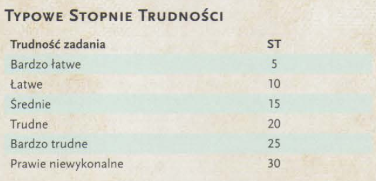
\includegraphics[width=1\textwidth]{test_sporny.png}
\end{figure}
\begin{figure}[h]
    \centering
    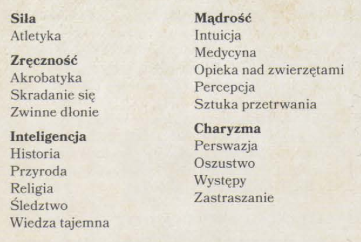
\includegraphics[width=1\textwidth]{umiejetnosci.png}
\end{figure}
\newpage

\subsection*{EFEKTY (STR. 290)}
\Centering
\textbf{NIEPRZYTOMNY}
\begin{itemize}
    \item Nieprzytomne stworzenie jest traktowane jak obezwładnione (zobacz opis stanu), nie może się poruszać ani mówić i nie ma świadomości tego, co się wokół niego dzieje.
    \item Stworzenie upuszcza wszystkie trzymane przedmioty i upada.
    \item Nieprzytomny automatycznie nie zdaje rzutów obronnych na Silę i Zręczność.
    \item Rzuty na atak przeciwko nieprzytomnemu są wykonywane z ułatwieniem.
    \item Każde trafienie w nieprzytomnego jest trafieniem krytycznym, jeśli atakujący znajduje się do 1,5 metra od celu.
\end{itemize}

\textbf{NIEWIDZIALNY}
\begin{itemize}
    \item Niewidzialnego stworzenia nie można zobaczyć bez zastosowania specjalnych zdolności lub magii. W przypadku ukrywania się niewidzialne stworzenie traktowane jest jak przebywające na obszarze pozbawionym widoczności. Jego obecność i lokalizację można ustalić na podstawie wydawanych przez nie dźwięków lub pozostawianych śladów.
    \item Testy ataku przeciwko niewidzialnemu stworzeniu są wykonywane z utrudnieniem, a niewidzialne stworzenie ma ułatwienie w testach ataku.
\end{itemize}

\textbf{OBEZWŁADNIONY}
\begin{itemize}
    \item Obezwładniona istota nie może podejmować akcji i reakcji.
\end{itemize}

\textbf{OGŁUCHŁY}
\begin{itemize}
    \item Ogluchla istota nie słyszy i automatycznie nie zdaje testów cech opartych na słuchu.
\end{itemize}

\textbf{OGŁUSZONY}
\begin{itemize}
    \item Ogłuszone stworzenie jest obezwładnione (zobacz opis stanu), nie może się poruszać i ma trudności z mówieniem.
    \item Stworzenie automatycznie nie zdaje rzutów obronnych na Silę i Zręczność.
    \item Testy ataku przeciwko ogłuszonemu stworzeniu są wykonywane z ułatwieniem.
\end{itemize}
\newpage

\textbf{OŚLEPIONY}
\begin{itemize}
    \item Oślepione stworzenie nie widzi i automatycznie nie zdaje testów cech opartych na wzroku.
    \item Testy ataku przeciwko oślepionemu stworzeniu wykonywane są z ułatwieniem, a oślepione stworzenie atakuje z utrudnieniem.
\end{itemize}

\textbf{POCHWYCONY}
\begin{itemize}
    \item Szybkość pochwyconego stworzenia spada do 0 i nie może ono korzystać z premii do szybkości.
    \item Stan pochwycenia kończy się, jeśli chwytający zostaje obezwładniony (zobacz opis stanu).
    \item Stan pochwycenia kończy się także, jeśli jakiś efekt spowoduje usunięcie pochwyconego stworzenia z zasięgu stoty chwytającej lub z obszaru efektu powodującego ten stan, na przyklad gdy zostanie odrzucone falą gromu.
\end{itemize}

\textbf{POWALONY}
\begin{itemize}
    \item Powalone stworzenie w ramach ruchu może tylko się czołgać, chyba że się podniesie i tym samym zakończy ten stan.
    \item Stworzenie ma utrudnienie w testach ataku.
    \item Test ataku przeciwko powalonemu jest wykonywany z ułatwieniem, o ile atakujący znajduje się do 1,5 metra od celu. W innym wypadku atak wykonywany jest z utrudnieniem.
\end{itemize}

\textbf{PRZERAŻONY}
\begin{itemize}
    \item Przerażone stworzenie wykonuje z utrudnieniem wszystkie testy cech i testy ataku, jeśli źródło jego strachu znajduje się w zasięgu wzroku.
    \item Przerażone stworzenie nie może z własnej woli zbliżyć się do źródła swego strachu.
\end{itemize}
\newpage

\textbf{SKAMIENIAŁY}
\begin{itemize}
    \item Skamieniale stworzenie wraz ze wszystkimi noszo- nymi lub trzymanymi niemagicznymi przedmiotami zostaje zmienione w nieruchomą, litą statuę (zazwyczaj kamienną). Stworzenie przestaje się starzeć, a jego waga rośnie dziesięciokrotnie.
    \item Stworzenie jest obezwładnione (zobacz opis stanu), nie może się poruszać ani mówić i nie ma świadomości tego, co się wokół niego dzieje.
    \item Testy ataku przeciwko skamieniałemu są wykonywane z ułatwieniem.
    \item Skamienialy automatycznie nie zdaje rzutów obronnych na Silę i Zręczność.
    \item Skamieniały zyskuje odporność na wszystkie rodzaje obrażeń.
    \item Skamieniale stworzenie jest niepodatne na trucizny i choroby, choć jeśli było już pod wypływem trucizny lub choroby, to nie zostaje ona zneutralizowana, a tylko wstrzymana.
\end{itemize}

\textbf{SPARALIŻOWANY}
\begin{itemize}
    \item Sparaliżowane stworzenie jest obezwładnione (zobacz opis stanu), a także nie może się ruszać ani mówić. Sparaliżowany automatycznie nie zdaje rzutów obron- nych na Silę i Zręczność.
    \item Testy ataku przeciwko sparaliżowanemu są wykonywane z ulatwieniem.
    \item Każde trafienie w sparaliżowanego jest trafieniem kry- tycznym, jeśli atakujący znajduje się do 1,5 metra od celu.
\end{itemize}

\textbf{UNIERUCHOMIONY}
\begin{itemize}
    \item Szybkość unieruchomionego stworzenia spada do 0 i nie może ono korzystać z premii do szybkości.
    \item Testy ataku przeciwko unieruchomionemu stworzeniu są wykonywane z ulatwieniem, a unieruchomione stworze- nie atakuje z utrudnieniem.
    \item Unieruchomione stworzenie ma utrudnienie w rzutach obronnych na Zręczność.
\end{itemize}

\textbf{ZATRUTY}
\begin{itemize}
    \item Zatrute stworzenie ma utrudnienie w rzutach na atak i testach cech.
\end{itemize}
\newpage

\textbf{ZAUROCZONY}
\begin{itemize}
    \item Zauroczone stworzenie nie może zaatakować istoty powodującej zauroczenie lub w inny sposób jej zaszkodzić (na przykład zaklęciami lub zdolnościami).
    \item Istota powodująca zauroczenie ma ułatwienie we wszystkich testach podczas interakcji społecznych z zauroczo- nym stworzeniem.
\end{itemize}
\textbf{WYCZERPANIE}
\begin{figure}[ht]
    \centering
    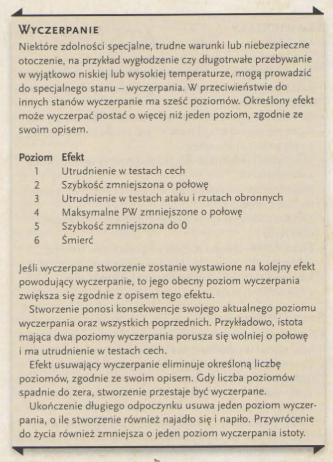
\includegraphics[width=0.75\textwidth]{wyczerpanie.png}
\end{figure}
\newpage

\end{document}